% Additional styles
\tikzstyle{block} = [rectangle, draw, text width=8em, text=white, text centered, rounded corners, minimum height=4em]
    
\tikzstyle{line} = [draw, -latex]

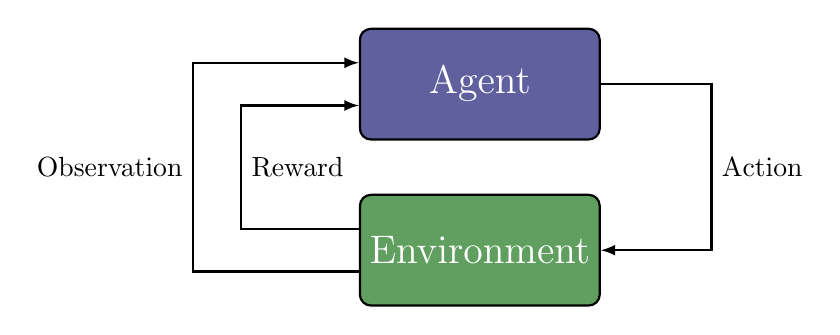
\begin{tikzpicture}[node distance = 6em, auto, thick]
    \node [block, fill=blue!25!gray] (Agent) {\Large Agent};
    \node [block, below of=Agent, fill=green!25!gray] (Environment) {\Large Environment};
    
     \path [line] (Agent.0) --++ (4em,0em) |- node [near start]{Action} (Environment.0);
     \path [line] (Environment.190) --++ (-6em,0em) |- node [near start] {Observation} (Agent.170);
     \path [line] (Environment.170) --++ (-4.25em,0em) |- node [near start, right] {Reward} (Agent.190);
\end{tikzpicture}
